\section{Auswertung}
    \subsection{Untergrundzählrate}
        Zuerst wird die Untergrundzählrate, die von jeder Messung abgezogen werden muss, um korrekte Messwerte zu bekommen.
        Deshalb wurden Werte für die Untergrundrate jeweils mit einer Integrationszeit von 300s gemessen:
        \begin{equation*}
            N_U = \{129, 143, 144, 136, 139, 126, 158\}
        \end{equation*}

        Der Mittelwert dieser Werte ist $N_{\text{U,m}} = (139 \pm 10)\,$Imp/300s. Da die Zählraten der Proben jedoch mit verschiedenen Integrationszeiten gemessen wurden, muss der Mittelwert auf diese Zeiten angepasst werden.

    \subsection{Vanadium}
        Da bei dieser Messreihe eine Messzeit von $\Delta t = 30$s verwendet wurde, wird die Untergrundzählrate durch 10 geteilt und von den gemessenen Werten $N^*_{\Delta t}$ abgezogen:
        \begin{equation*}
            N_{\Delta t} = N^*_{\Delta t} - \frac{N_{\text{U,m}}}{10}
        \end{equation*}
        
        Die Messwerte werden halblogarithisch aufgetragen. Nach \autoref{eqn:theorieGerade} sollten die Werte theoretisch ca. proportional zur Zerfallskonstante $\lambda$ sein:
        \begin{align*}
            &\underbrace{\ln\left(N_{\Delta t}(t)\right)} = \underbrace{\ln \left(N_0 \cdot \left(1 - e^{-\lambda \Delta t}\right)\right)} \underbrace{ - \lambda} \hspace{2pt} \cdot \hspace{3pt} \underbrace{t} \\
            & \hspace{26pt} y \hspace{25pt} = \hspace{47pt} b \hspace{49pt} + m \cdot x
        \end{align*}            

        Deshalb kann eine lineare Regression durch alle Werte durchgeführt werden, um die Zerfallskonstante und damit auch die Halbwertszeit anhand von \autoref{eqn:Halbwertszeit} zu berechnen.
        Es ist jedoch leicht in \autoref{fig:Vanadium} zu erkennen, dass die Messwerte aufgrund der halblogarithmischen Darstellungsweise stark divergieren.

        Deswegen wird zuerst mithilfe der ersten linearen Regression die vorläufige Halbwertszeit $T_{\nicefrac{1}{2}}$ bestimmt und für die zweite lineare Regression werden nur die Messwerte bis ca. zur doppelten Halbwertszeit, in diesem Fall die ersten 14, verwendet.

        \begin{figure}[h]
            \centering
            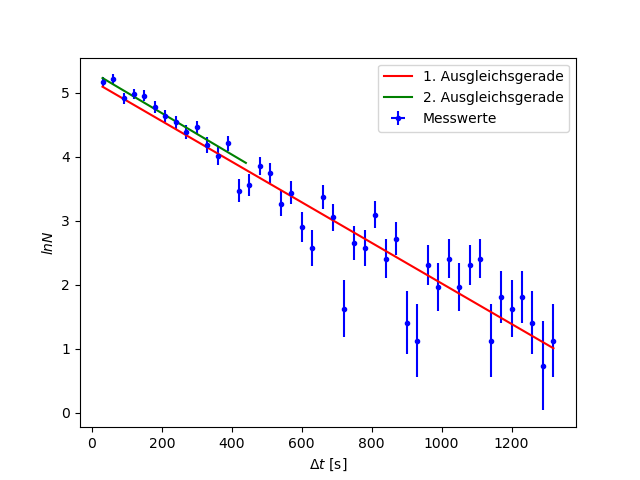
\includegraphics[width = 0.8\textwidth]{pictures/HalbwertszeitGraph_Vanadium.png}
            \caption{Es sind die Werte aus \autoref{tab:Vanadium} halblogarithmisch aufgetragen und eine Ausgleichgerade wird zuerst durch alle Punkte und eine zweite Ausgleichsgerade durch die ersten 14 Werte durchgeführt.}
            \label{fig:Vanadium}
        \end{figure}

        \FloatBarrier

        Für die erste und zweite Ausgleichsgerade ergeben sich folgende Werte:
        \begin{align*}
            m_1 = (-3,17 \pm 0,16 \cdot 10^{-3}) \text{s}^{-1} \hspace{75pt} b_1 = (5,19 \pm 0,13) \\
            m_2 = (-3,23 \pm 0,24 \cdot 10^{-3}) \text{s}^{-1} \hspace{75pt} b_2 = (5,32 \pm 0,06)
        \end{align*}

        Also ergibt sich mit \autoref{eqn:Halbwertszeit} für die Halbwertszeiten
        \begin{align*}
            T_{\nicefrac{1}{2} \text{, 1}} = (219 \pm 11)\, \text{s} \\
            T_{\nicefrac{1}{2} \text{, 2}} = (214 \pm 16)\, \text{s}
        \end{align*}
        und aus dem y-Achsenabschnitt werden die Vorfaktoren
        \begin{align*}
            \text{e}^{b_1} = N_0 \left(1 - e^{-\lambda_1 \Delta t}\right) = (178 \pm 23) \,\text{Imp} \\
            \text{e}^{b_2} = N_0 \left(1 - e^{-\lambda_2 \Delta t}\right) = (205 \pm 12) \,\text{Imp}
        \end{align*}
        berechnet.

        Die Abweichung der Halbwertszeit vom Literaturwert $T_{\nicefrac{1}{2} \text{,lit}} = 224,6 \,$s sind:
        \begin{align*}
            a_1 = \frac{T_{\nicefrac{1}{2} \text{,lit}} - T_{\nicefrac{1}{2} \text{, 1}}}{T_{\nicefrac{1}{2} \text{,lit}}} = 2,6 \, \% \\
            a_2 = \frac{T_{\nicefrac{1}{2} \text{,lit}} - T_{\nicefrac{1}{2} \text{, 2}}}{T_{\nicefrac{1}{2} \text{,lit}}} = 4,5 \, \%
        \end{align*}

    \newpage
    \subsection{Rhodium}
        Bei dem Zerfall von Rhodium besteht das Problem, dass gleichzeitig zwei verschiedene Zerfallsprozesse stattfinden (siehe \autoref{eqn:Rhodium}).

        Davon läuft der Eine langsamer und der Andere schneller ab. Deshalb sind nach einer gewissen Zeit $t^*$ in der Messung alle schnellen Zerfallsprozesse abgelaufen und es bleibt nur noch der langsame Zerfall. Das kann ist gut in \autoref{fig:Rhodium} daran erkennbar, dass der Graph zuerst schnell fällt und dann ab ca. $t^*$ einen linearen Anteil aufweist.

        Es wird also zuerst die lineare Regression durch den linearen Teil des Graphen gemacht. Bei diesem Fall wurden die 18 letzten Messwerte benutzt.

        Dann wird die Ausgleichsgerade extrapoliert und von dem Graphen subtrahiert. Dabei ist darauf zu achten, dass alle Werte der Ausgleichsgeraden unterhalb der Werten $N_{\Delta t}(t)$ mit $t < t^*$ liegen.
        \begin{figure}[h]
            \centering
            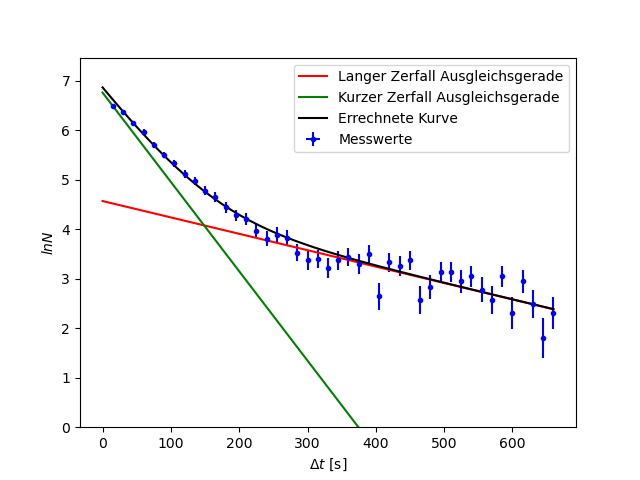
\includegraphics[width = 0.8\textwidth]{pictures/HalbwertszeitGraph_Rhodium.png}
            \caption{Es sind die Werte aus \autoref{tab:Rhodium} halblogarithmisch aufgetragen und eine Ausgleichgerade durch die letzten 18 Werte durchgeführt. Anschließend wird eine Ausgleichsgerade durch die ersten 14 korrigierten Werte durchgeführt.}
            \label{fig:Rhodium}
        \end{figure}

        \FloatBarrier
        
        Aus den Parametern der Ausgleichsgerade für den langsamen Zerfall
        \begin{equation*}
            m_l = (-3,31 \pm 1,00 \cdot 10^{-3}) \text{s}^{-1} \hspace{75pt} b_l = (4,57 \pm 0,54)
        \end{equation*}

        ergibt sich mit der gleichen Rechnung wie beim Vanadium die Halbwertszeit $T_{\nicefrac{1}{2} \text{, l}} = (209 \pm 63) \,$s und der Vorfaktor $e^{b_l} = (96,5 \pm 51,8) \,$Imp. \\

        Wie in \autoref{fig:Rhodium} zu erkennen ist, macht es keinen Sinn die Ausgleichsgerade in einen Graphen einzuzeichnen, in dem der langsame Zerfall noch vorhanden ist.
        \begin{figure}[h]
            \centering
            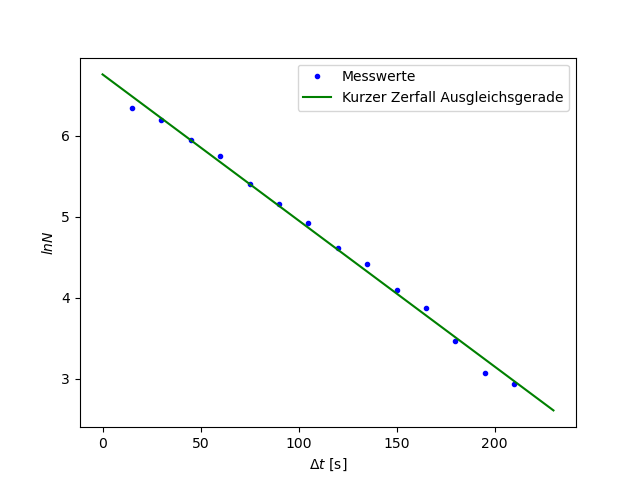
\includegraphics[width = 0.8\textwidth]{pictures/HalbwertszeitGraph_Rhodium_kurzlebig.png}
            \caption{Es sind die ersten 14 Werte aus \autoref{tab:Rhodium} halblogarithmisch aufgetragen, nachdem der langsame Zerfall abgezogen wurde.}
            \label{fig:RhodiumSchnell}
        \end{figure}

        \FloatBarrier

        Aus den Parametern der Ausgleichsgerade für den schnellen Zerfall
        \begin{equation*}
            m_s = (-18,1 \pm 0,4 \cdot 10^{-3}) \text{s}^{-1} \hspace{75pt} b_s = (6,76 \pm 0,05)
        \end{equation*}

        ergibt sich mit der gleichen Rechnung wie beim Vanadium die Halbwertszeit $T_{\nicefrac{1}{2} \text{, s}} = (38,4 \pm 0,8)$ und der Vorfaktor $e^{b_s} = (862,8 \pm 41) \,$Imp. \\

        Die Abweichung der Halbwertszeit des langsamen und schnellen Zerfalls von den Literaturwerten $T_{\nicefrac{1}{2} \text{,l,lit}} = 260,4 \,$s und $T_{\nicefrac{1}{2} \text{,s,lit}} = 42,3 \,$s sind jeweils:
        \begin{align*}
            &a_l = 19,6 \, \% \\
            &a_s = 9,2 \, \%
        \end{align*}

        Die Theoriekurve in \autoref{fig:Rhodium} wurde mit den jetzt bekannten Werten für die Zerfallskonstanten gezeichnet, anhand folgender Formel, die aus der Summe der beiden Gleichungen \ref{eqn:Zerfallsgesetz_} für den langsamen Zerfall und schnellen Zerfall entsteht:
        \begin{align*}
            &&N_{\Delta t, ges} &= N_0 (1 - e^{-\lambda_l \Delta t}) \cdot e^{-\lambda_l t} + N_0 (1 - e^{-\lambda_s \Delta t}) \cdot e^{-\lambda_s t} \\
            \implies &&\ln\Bigl(N_{\Delta t, ges} \Bigr) &= \ln\Bigl(N_0 (1 - e^{-\lambda_l \Delta t}) \cdot e^{-\lambda_l t} + N_0 (1 - e^{-\lambda_s \Delta t}) \cdot e^{-\lambda_s t} \Bigr)
        \end{align*}

